% Part: sets-functions-relations
% Chapter: relations
% Section: trees
% Hindi translation (hi-Deva-IN) of Open Logic commit 9620cc73f9c8e0ad003c514a5d3748f29611c4c0.

\documentclass[../../../include/open-logic-section]{subfiles}

\begin{document}

\olfileid[hi]{sfr}{rel}{tre}
\olsection{वृक्ष}

आंशिक क्रम का एक विशेष प्रकार, जिसकी तर्कशास्त्र के सभी भागों में महत्त्वपूर्ण
भूमिका है, \emph{वृक्ष} कहलाता है। परिमित वृक्ष तर्कशास्त्र के आरंभिक भागों
में मिलते हैं: उदाहरणार्थ, !!{formula}s को वाक्यविन्यास-वृक्ष में उनके विघटन
के आधार पर समझा जा सकता है, जबकि अनेक !!{derivation} पद्धतियों में
!!{derivation}s भी परिमित वृक्षों का रूप लेते हैं।
%
अनंत वृक्ष प्रतिज्ञप्तिक और प्रथम-कोटि तर्कशास्त्र के पूर्णता प्रमेयों के
प्रमाण में ही सामने आ जाते हैं, और गणितीय तर्कशास्त्र में सर्वत्र प्रयुक्त
होते हैं।

वृक्ष की समुच्चय-सैद्धान्तिक संकल्पना आलेख सिद्धान्त में वृक्ष की धारणा से
निकटतः संबंधित है। यहाँ एक (परिमित) वृक्ष का चित्र है:

\begin{center}
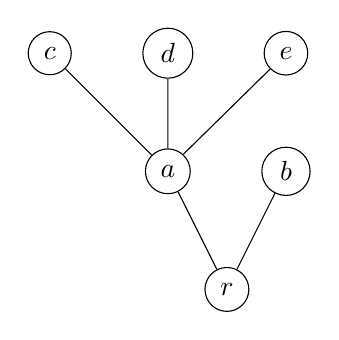
\begin{tikzpicture}[nodes={draw, circle}, -]
\node{$r$} [grow'=up]
    child { node {$a$} 
        child { node {$c$} }
        child { node {$d$} }
        child { node {$e$} }
    }
    child { node {$b$} };
\end{tikzpicture}
\end{center}

सबसे नीचे का संधि-बिंदु~$r$ मूल है। $r$ को छोड़कर प्रत्येक संधि-बिंदु का ठीक
एक जनक संधि-बिंदु उसके ठीक नीचे होता है। किसी संधि-बिंदु~$x$ और किसी
संधि-बिंदु~$y$ के बीच उस संबंध में, जिसमें कोरों का ऊपर की ओर अनुसरण करके
$y$ तक~$x$ से पहुँचा जा सकता है, हम कह सकते हैं कि~$x$,~$y$ का
\emph{पूर्वज} है।

वृक्ष में पूर्वज-संबंध एक प्रबल आंशिक क्रम है। यही समुच्चय-सैद्धान्तिक
परिभाषा की प्रेरणा देता है। उसे बताने के लिए हमें दो संकल्पनाएँ चाहिए।
समुच्चय~$A$ को~$\le$ द्वारा आंशिक रूप से क्रमित किए जाने पर उसमें
\emph{न्यूनतम अवयव} ऐसा !!a{element} $x \in A$ है कि प्रत्येक $y \in A$
के लिए~$x \le y$ हो। किसी समुच्चय को~$\le$ द्वारा \emph{सुक्रमित} तब कहते
हैं जब उसके प्रत्येक अरिक्त उपसमुच्चय में न्यूनतम अवयव हो।

\begin{defn}[वृक्ष]
\emph{वृक्ष} ऐसा युग्म $T = \tuple{A, \le}$ है कि $A$ एक समुच्चय है और
$\le$,~$A$ पर एक आंशिक क्रम है, जिसका एक अद्वितीय न्यूनतम अवयव
$r \in A$ है (जिसे \emph{मूल} कहते हैं), तथा प्रत्येक $x \in A$ के लिए
समुच्चय $\Setabs{y}{y \le x}$,~$\le$ द्वारा सुक्रमित है।
\end{defn}

\begin{defn}[उत्तरवर्ती]
मान लीजिए कि $T = \tuple{A, \le}$ एक वृक्ष है।
यदि $x,y \in A$, $x < y$, और ऐसा कोई $z \in A$ नहीं है कि
$x < z < y$, तो हम $y$ को~$x$ का \emph{उत्तरवर्ती} कहते हैं।
\end{defn}

$x \in A$ के उत्तरवर्तियों को उसकी \emph{संतानें} भी कहते हैं। यदि
$y$,~$x$ का उत्तरवर्ती है, तो हम $x$ को~$y$ का \emph{पूर्ववर्ती} या
\emph{जनक} कहते हैं।

\begin{prop}
यदि $\tuple{A,\le}$ एक वृक्ष है, तो मूल को छोड़कर प्रत्येक $x \in A$ का
अधिकतम एक पूर्ववर्ती है।
\end{prop}

\begin{proof}
  मान लीजिए कि $y_1 < x$ और $y_2 < x$ तथा $y_1 \neq y_2$। तब $\{y_1,
  y_2\} \subseteq \Setabs{z}{z<x}$। चूँकि $\Setabs{z}{z<x}$,
  $\le$ द्वारा सुक्रमित है, इसलिए उसके उपसमुच्चय $\{y_1, y_2\}$ में एक
  न्यूनतम अवयव है, जो स्पष्टतः $y_1$ या~$y_2$ ही होगा। अतः या तो
  $y_1 \le y_2$ या $y_2 \le y_1$। हमने माना है कि $y_1 \neq y_2$, इसलिए
  वास्तव में या तो $y_1 < y_2$ या $y_2 < y_1$। चूँकि हमने $y_1 < x$ और
  $y_2 < x$ भी माना है, इसलिए आगे या तो $y_1 < y_2
  < x$ या
  $y_2 < y_1 < x$। अतः $y_1$ और $y_2$ दोनों~$x$ के पूर्ववर्ती नहीं हो
  सकते।
\end{proof}

\begin{defn}
वृक्ष $T = \tuple{A, \le}$ को \emph{अनंत} कहते हैं यदि $A$ एक अनंत
समुच्चय है, और अन्यथा उसे \emph{परिमित} कहते हैं। यदि $T$ ऐसा है कि प्रत्येक
$x \in A$ के केवल परिमित रूप से अनेक उत्तरवर्ती हैं, तो हम $T$ को
\emph{परिमित-शाखी} कहते हैं।
\end{defn}

\begin{defn}[शाखाएँ]
दिए गए वृक्ष $T = \tuple{A, \le}$ के लिए,~$T$ की \emph{शाखा},~$T$ में एक
अधिकतम शृंखला है; अर्थात ऐसा समुच्चय $B \subseteq A$ कि किन्हीं
$x, y \in B$ के लिए या तो $x \le y$ या $y \le x$, और प्रत्येक
$z \in X \setminus B$ के लिए ऐसा $u \in B$ विद्यमान हो कि न तो
$z \le u$ और न $u \le z$।
%
हम $[T]$ का प्रयोग $T$ की सभी शाखाओं के समुच्चय को दर्शाने के लिए करते हैं।
\end{defn}

\begin{ex}
परिमित-शाखी वृक्ष का एक प्रसिद्ध उदाहरण $0$ और~$1$ के परिमित अनुक्रमों का
\emph{अनंत द्विआधारी वृक्ष} है, जिसे कभी-कभी $\{0,1\}^*$ या~$\Bin^*$
लिखते हैं और विस्तार संबंध $\sqsubseteq$ द्वारा क्रमित करते हैं
(उदाहरणतः $101 \sqsubseteq 101101$)। चूँकि किसी भी द्विआधारी वर्ण-शृंखला
के अंत में $0$ या $1$ जोड़कर उसका विस्तार हमेशा किया जा सकता है, इसलिए इस
वृक्ष में अनंत रूप से अनेक अवयव हैं: प्रत्येक अवयव~$s$ के ठीक दो उत्तरवर्ती,
$s0$ और~$s1$, हैं। इसका मूल रिक्त अनुक्रम $\emptyseq$ है।
\end{ex}

\begin{ex}
कुछ और सामान्य रूप में, प्राकृत संख्याओं के परिमित अनुक्रमों का
समुच्चय~$\Nat^*$, जिसे विस्तार संबंध~$\sqsubseteq$ से क्रमित किया गया है,
भी एक वृक्ष है। यह स्पष्टतः
परिमित-शाखी नहीं है: प्रत्येक $s \in \Nat^*$ के अनंत रूप से अनेक
उत्तरवर्ती~$sn$ हैं, प्रत्येक $n \in \Nat$ के लिए एक। प्रत्येक
$A
\subseteq \Nat^*$ जो~$\sqsubseteq$ के अधीन संवृत है,~$\Nat^*$ का
\emph{उपवृक्ष} है। (अर्थात $A$ ऐसा है कि यदि $s \in A$ और
$s' \sqsubseteq s$, तो $s' \in A$ भी।) सभी परिमित वृक्षों को~$\Nat^*$ के
परिमित उपवृक्षों के रूप में निरूपित किया जा सकता है।
\end{ex}

\begin{prop}[K\H{o}nig का उपप्रमेय]
यदि $T = \tuple{A,\le}$ एक परिमित-शाखी अनंत वृक्ष है, तो $T$ की एक अनंत
शाखा है।
\end{prop}

संगणनीयता सिद्धान्त में व्यापक रूप से प्रयुक्त K\H{o}nig के उपप्रमेय का एक
विशेष रूप, जिसे \emph{दुर्बल K\H{o}nig उपप्रमेय} कहते हैं, यह है:
$\{0,1\}^*$ के प्रत्येक अनंत उपवृक्ष की एक अनंत शाखा होती है।

\end{document}
